%%% Template originaly created by Karol Kozioł (mail@karol-koziol.net) and modified for ShareLaTeX use

\documentclass[a4paper,11pt,pagenumber=true]{article}

\usepackage{graphicx,url}
\usepackage[brazil]{babel}   
\usepackage[utf8]{inputenc}  
\usepackage{dirtytalk}
\usepackage{verbatim}
\usepackage{listings}
\usepackage{xcolor}

%\renewcommand\familydefault{\sfdefault}
%\usepackage{tgheros}
%\usepackage[defaultmono]{droidmono}

\usepackage{pifont,textcomp,gensymb}
\usepackage{amsmath,amssymb,amsthm}
\usepackage{enumerate, multicol}
\usepackage{tikz, booktabs}

\usepackage{geometry}
\geometry{
    total={210mm,297mm},
    left=25mm,right=25mm,
    bindingoffset=0mm, 
    top=20mm,bottom=20mm
}
\linespread{1.3}

\newcommand{\linia}{\rule{\linewidth}{0.5pt}}

% vectors specification shortcuts.
\newcommand{\veci}{$\mathbf{u}$}
\newcommand{\vecj}{$\mathbf{v}$}
\newcommand{\veck}{$\mathbf{w}$}

% other math shortcuts. Use only on math mode.
\newcommand{\vecnorm}[1]{\|\mathbf{#1}\|}
\newcommand{\dotprod}[2]{\mathbf{#1} \bullet \mathbf{#2}}
\newcommand{\sen}{\text{\,sen\,}}

\newtoks\institution

% custom theorems if needed
\newtheoremstyle{mytheor}
    {1ex}{1ex}{\normalfont}{0pt}{\scshape}{.}{1ex}
    {{\thmname{#1 }}{\thmnumber{#2}}{\thmnote{ (#3)}}}
\theoremstyle{mytheor}
\newtheorem{defi}{Definition}

% my own titles
\makeatletter
\renewcommand{\maketitle}{
    \begin{center}
        \vspace{2ex}
        {\huge \textsc{\@title}}
        \vspace{1ex}\\
        \linia\\
        \@author\\ 
        \linia\\
        \vspace{1ex}
        \textsc{\the\institution} 
        \hfill \@date
        \vspace{4ex}
    \end{center}
}
\makeatother
%%%

% custom footers and headers
\usepackage{fancyhdr}
\pagestyle{fancy}
\lhead{}
\chead{}
\rhead{}
\lfoot{Lista de Exercícios de Computação Gráfica \textnumero{2}}
\cfoot{}
\rfoot{Página \thepage}
\renewcommand{\headrulewidth}{0pt}
\renewcommand{\footrulewidth}{0pt}
%

% code listing settings
\usepackage{listings}
\renewcommand{\lstlistingname}{Listagem}
\renewcommand{\lstlistlistingname}{Relação de \lstlistingname s}
\lstset{
    language=R,
    basicstyle=\ttfamily\small,
    aboveskip={1.0\baselineskip},
    belowskip={1.0\baselineskip},
    columns=fixed,
    extendedchars=true,
    breaklines=true,
    tabsize=4,
    prebreak=\raisebox{0ex}[0ex][0ex]{\ensuremath{\hookleftarrow}},
    frame=lines,
    showtabs=false,
    showspaces=false,
    showstringspaces=false,
    keywordstyle=\color[rgb]{0.627,0.126,0.941},
    commentstyle=\color[rgb]{0.133,0.545,0.133},
    stringstyle=\color[rgb]{01,0,0},
    numbers=left,
    numberstyle=\small,
    stepnumber=1,
    numbersep=10pt,
    captionpos=t,
    escapeinside={\%*}{*)},
    literate={á}{{\'a}}1 {â}{{\^a}}1 {ã}{{\~a}}1 {à}{{\`a}}1 {é}{{\'e}}1 {ê}{{\^e}}1 {ó}{{\'o}}1 {ô}{{\^o}}1 {õ}{{\~o}}1 {ú}{{\'u}}1 {~}{{\~}}1 {é}{{\'e}}1 {ç}{{\,c}}1 {í}{{\'i}}1
}

%%%----------%%%----------%%%----------%%%----------%%%

\begin{document}

    \title{Lista de Exercícios de\\Computação Gráfica \textnumero{2}}

    \author{Jonas de Araújo Luz Jr.\\
    unifor@jonasluz.com}
    \institution{Profa. Andreia Formico}
    \date{09/03/2017}
    
    \begin{figure}[t]
    \centering
        
\includegraphics[width=.2\textwidth]{images/logo-UNIFOR.jpg}
        \label{fig:logo}    
    \end{figure}
    
    \maketitle
    \tableofcontents
    \newpage
    
    \section{Questão \textnumero{1}}
    
        Elimine o parâmetro $u$ da seguinte equação vetorial: $\mathbf{r}(u) = au^2 \mathbf{i} + 2au \mathbf{j}$, onde $a$ é um valor escalar. Verifique que esta equação vetorial corresponde à parábola cuja equação cartesiana é $y^2 = 4ax$.
        
        \subsection*{Solução:}
        
            Tomando a equação vetorial dada, temos que: 
            \begin{equation*}
                \begin{matrix}
                    x = au^2 \\
                    y = 2au
                \end{matrix}
            \end{equation*}
            
            Colocando u em função de $x$ e fazendo a substituição na equação de $y$, obtemos:
            \[u = \sqrt{\frac{x}{a}}\]
            \[y = 2a\left(\sqrt{\frac{x}{a}}\right)\]
            
            Elevando ambos os lados desta equação ao quadrado, fica:
            \[
                y^2 = 4a^2\left(\frac{x}{a}\right) \implies
                y^2 = 4ax
            \] conforme queríamos demonstrar. 
            
            Ilustramos a equação parabólica para diferentes valores de $a$ na Figura \ref{fig:q1}.

            \begin{figure}[h]
            \centering
            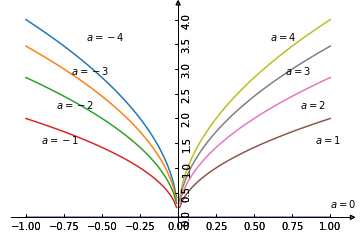
\includegraphics[width=.9\textwidth]{images/q-1.png}
                \label{fig:q1}
                \caption{Gráfico de $y^2 = 4ax$}
            \end{figure}

    \section{Questão \textnumero{2}}
    
        Considere a curva planar dada pela equação vetorial: $\mathbf{r}(u) = -u \mathbf{i} + \frac{1}{u} \mathbf{j}, u \neq 0$. Construa uma tabela de valores para $u$ e, então, esboce esta curva para $-10 \leq u \leq 10$. Inclua considerações sobre $-1 < u < 0$ e $0 < u < 1$. 
    
        \subsection*{Solução}
            
            As equações paramétricas correspondentes à vetorial dada são: 
            \begin{equation*}
                \begin{matrix}
                    x = -u \\
                    y = \frac{1}{u}
                \end{matrix} \\
                \text{ para } u \neq 0
            \end{equation*}
            
            Disto, temos que quando $u \neq 0$, então $x \neq 0$.
            
            Agora, colocando $y$ em função de $x$, obtemos: 
            \begin{equation} \label{eq:2}
                y = -\frac{1}{x} \text{ para } x \neq 0
            \end{equation}
            
            A Tabela \ref{tab:21} apresenta os valores para $u$ variando de -10 a 10, necessário para desenho do gráfico da equação vetorial. Os valores de $u$ variando de -1 a 1 são apresentados na Tabela \ref{tab:22}.
            % Tabela com valores de u de -10 a 10.
            \begin{table}[h]
                \centering
                \begin{tabular}{c|c|c|c}
                    \toprule
                        $u$	&$x$	&$y$	&$\mathbf{r}(u)$\\ \midrule
                        -10	& 10	& -0.10	&$10\mathbf{i} -   0.10\mathbf{j}$\\
                         -9	&  9	& -0.11	&$9\mathbf{i} -   0.11\mathbf{j}$\\
                         -8	&  8	& -0.12	&$8\mathbf{i} -   0.12\mathbf{j}$\\
                         -7	&  7	& -0.14	&$7\mathbf{i} -   0.14\mathbf{j}$\\
                         -6	&  6	& -0.17	&$6\mathbf{i} -   0.17\mathbf{j}$\\
                         -5	&  5	& -0.20	&$5\mathbf{i} -   0.20\mathbf{j}$\\
                         -4	&  4	& -0.25	&$4\mathbf{i} -   0.25\mathbf{j}$\\
                         -3	&  3	& -0.33	&$3\mathbf{i} -   0.33\mathbf{j}$\\
                         -2	&  2	& -0.50	&$2\mathbf{i} -   0.50\mathbf{j}$\\
                         -1	&  1	& -1.00	&$1\mathbf{i} -   1.00\mathbf{j}$\\
                          1	& -1	&  1.00	&$-1\mathbf{i} +   1.00\mathbf{j}$\\
                          2	& -2	&  0.50	&$-2\mathbf{i} +   0.50\mathbf{j}$\\
                          3	& -3	&  0.33	&$-3\mathbf{i} +   0.33\mathbf{j}$\\
                          4	& -4	&  0.25	&$-4\mathbf{i} +   0.25\mathbf{j}$\\
                          5	& -5	&  0.20	&$-5\mathbf{i} +   0.20\mathbf{j}$\\
                          6	& -6	&  0.17	&$-6\mathbf{i} +   0.17\mathbf{j}$\\
                          7	& -7	&  0.14	&$-7\mathbf{i} +   0.14\mathbf{j}$\\
                          8	& -8	&  0.12	&$-8\mathbf{i} +   0.12\mathbf{j}$\\
                          9	& -9	&  0.11	&$-9\mathbf{i} +   0.11\mathbf{j}$\\
                         10	&-10	&  0.10	&$-10\mathbf{i} +   0.10\mathbf{j}$\\
                    \bottomrule
                \end{tabular}
                \caption{Tabela de valores para $\mathbf{r}(u)$, com $u$ variando de -10 a 10}
                \label{tab:21}
            \end{table} 
            
            % Tabela com valores de u de -1 a 1.
            \begin{table}[h]
                \centering
                \begin{tabular}{c|c|c|c}
                    \toprule
                        $u$	&$x$	&$y$	&$\mathbf{r}(u)$\\ \midrule
                        -1.0	&   1.0	& -1.00	&$   1.0\mathbf{i} -   1.00\mathbf{j}$\\
                         -0.8	&   0.8	& -1.25	&$   0.8\mathbf{i} -   1.25\mathbf{j}$\\
                         -0.6	&   0.6	& -1.67	&$   0.6\mathbf{i} -   1.67\mathbf{j}$\\
                         -0.4	&   0.4	& -2.50	&$   0.4\mathbf{i} -   2.50\mathbf{j}$\\
                         -0.2	&   0.2	& -5.00	&$   0.2\mathbf{i} -   5.00\mathbf{j}$\\
                          0.2	&  -0.2	&  5.00	&$  -0.2\mathbf{i} +   5.00\mathbf{j}$\\
                          0.4	&  -0.4	&  2.50	&$  -0.4\mathbf{i} +   2.50\mathbf{j}$\\
                          0.6	&  -0.6	&  1.67	&$  -0.6\mathbf{i} +   1.67\mathbf{j}$\\
                          0.8	&  -0.8	&  1.25	&$  -0.8\mathbf{i} +   1.25\mathbf{j}$\\
                          1.0	&  -1.0	&  1.00	&$  -1.0\mathbf{i} +   1.00\mathbf{j}$\\
                    \bottomrule
                \end{tabular}
                \caption{Tabela de valores para $\mathbf{r}(u)$, com $u$ variando de -1 a 1}
                \label{tab:22}
            \end{table}
            
            O gráfico da equação de $\mathbf{r}(u)$, na forma da Equação \ref{eq:2} ($y$ em função de $x$), é apresentado na Figura \ref{fig:q2}. Observando-o com apoio da Tabela \ref{tab:22}, percebe-se que, no intervalo de $u$ variando de $[-1, 1]$, a curva aproxima-se, indefinidamente, dos eixos de coordenadas (ordenadas e abscissas), porém sem nunca tocá-los. Isto se deve ao fato de que a função $y \vdash f(x)$ (Equação \ref{eq:2}) definida sobre o intervalo $[-1, 1]$ não possui derivada em $x=0$, sendo seus valores quando $x= -1$ e $x = 1$ seus pontos extremos -- mínimo e máximo, respectivamente.
            
            \begin{figure}[h]
            \centering
                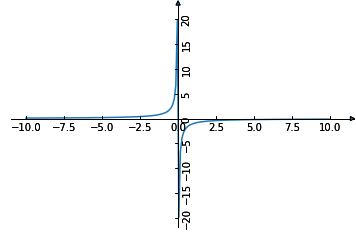
\includegraphics[width=.9\textwidth]{images/q-2.png}
                \label{fig:q2}
                \caption{Gráfico de $y = -\frac{1}{x}$}
            \end{figure}
        
            \clearpage
            
    \section{Questão \textnumero{3}}

        A curva 3D abaixo tem a seguinte equação vetorial: 
        $r(\theta) =    \frac{\theta}{360} \mathbf{ i} + 
                        5 \cos \theta \mathbf{ j} + 
                        3 \sen \theta \mathbf{ k}$
        , onde $\theta$ é medido em graus. Identifique esta curva e descreva suas principais características.

        \begin{figure}[h]
        \centering
            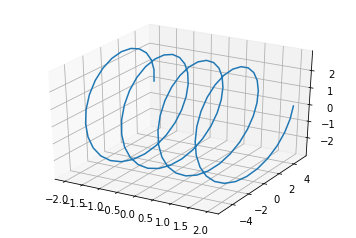
\includegraphics[width=.9\textwidth]{images/q-3.png}
            \label{fig:q3}
        \end{figure}        
        
        \subsection*{Solução}
        
            As equações paramétricas da curva são dadas por: 
            \[
                \begin{matrix}
                    x = \frac{\theta}{360}  \\
                    y = 5 \cos \theta       \\
                    z = 3 \sen \theta
                \end{matrix}
            \]
            
            Para eliminar $\theta$ das equações paramétricas de $y$ e $z$, escrevemos:
            \[
                \begin{matrix}
                    \frac{y^2}{5^2} = \cos^2 \theta \\
                    \frac{z^2}{3^2} = \sen^2 \theta
                \end{matrix}
            \]
            
            Somando membro a membro, obtemos:
            \[\frac{y^2}{5^2} + \frac{z^2}{3^2} = 1\]
            
            Logo, a curva é um \say{espiral} que está inteiramente no cilindro elíptico cuja diretriz é uma elipse no plano $yz$ cujas determinantes são paralelas ao eixo $x$. \cite{leitholdcalculo} \\
    
            O ponto onde a curva intercepta o eixo $yz$ pode ser determinado fazendo-se $x = 0$:
            \[
                \begin{matrix}
                    \frac{\theta}{360} = 0 \implies \theta = 0  \\
                    y = 5 \cos \theta = 5 \cos 0 = 5            \\
                    z = 3 \sen \theta = 3 \sen 0 = 0            \\
                    \\
                    P_0 = (0, 5, 0)
                \end{matrix}
            \]

            %%%
            \begin{comment} % Tentativa de derivar as equações das retas paramétricas da elipse diretriz da curva...

            As retas que limitam a elipse diretriz da curva ao longo do plano $xz$ podem ser determinadas, sabendo-se, nestas, temos $y = 0$: 
            \[y = 5 \cos \theta = 0 \implies \cos \theta = 0\]
            Os valores de $\theta$ que atendem a isto podem ser separados em dois domínios, $S_\theta$ e $S'_\theta$, tais que:
            \[
                \begin{matrix}
                    S_\theta  = \left\{ \theta = 90 + 360 b\,|\,b \in \mathbb{Z} \right\} \text{ e }    \\
                    S'_\theta = \left\{ \theta = 270 + 360 b\,|\,b \in \mathbb{Z} \right\}              \\
                \end{matrix}
            \]
            
            Tomando-se dois valores distintos de $b$, obtemos dois pontos em cada domínio acima e, a partir destes, as duas retas que limitam a elipse diretriz da curva ao longo do plano $xz$. Tomemos $b=0$ e $b=1$. Temos:
            \[
                \begin{matrix}
                    \text{Para } S:                             \\
                    \theta=90\degree\ \implies 
                    x=\frac{90}{360} = \frac{1}{4} \text{ e }   \\
                    z= 3 \sen 90 = 3                            \\
                    \text{Para } S':                            \\
                    \theta=2
                    \theta=270\degree
                \end{matrix}
            
            \]
            
            \end{comment}
            %%%
            
            As retas, paralelas ao eixo $x$, que limitam a elipse diretriz da curva são: 
            
            \[
                \begin{matrix}
                    \mathbf{D}_y = \frac{\theta}{360} \mathbf{i} + 5 \mathbf{j}     \\
                    \mathbf{D'}_y = \frac{\theta}{360} \mathbf{i} - 5 \mathbf{j}    \\
                    \mathbf{D}_z = \frac{\theta}{360} \mathbf{i} + 3 \mathbf{k}     \\
                    \mathbf{D'}_z = \frac{\theta}{360} \mathbf{i} - 3 \mathbf{k}    
                \end{matrix}
            \]
            
            A Figura \ref{fig:q3answer} ilustra a curva e as retas paralelas ao eixo $x$ que limitam a elipse diretriz da curva.
            
            \begin{figure}[h]
            \centering
                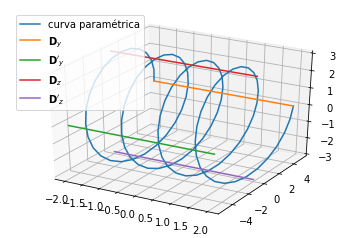
\includegraphics[width=.9\textwidth]{images/q-3answer.png}
                \label{fig:q3answer}
            \end{figure}        
            
\nocite{*}
\bibliographystyle{acm}
\bibliography{assignment}

\end{document}
